\section{Spark}

\subsection{Présentation générale}

Spark est un framework open-source qui permet de traiter de larges volumes de données. C'est un framework qui est utilisé pour de grosse volumétries de données (supérieur en taille à 1 To de données). Pour des faibles volumétries de données, il existe différents outils plus simple et plus léger à mettre en place.

\subsection{Usages}

Spark permet de répondre à différents cas d'utilisations :

\begin{itemize}
  \item Faire de l'analyse de logs
  \item Traiter des fichiers de texte
  \item Faire de la recommandations pour des produits, des articles ...
  \item Faire de la détection de fraude et de la sécurité
  \item Recherche distribuée (Google, Facebook ...)
\end{itemize}

\subsection{Aspect fondamentale}

Spark tourne au seins d'un cluster  :

\begin{itemize}
  \item Spark peut fonctionner de différentes façon au niveau de la gestion du cluster. Il pourra être en standalone ainsi se débrouiller de maniéres autonome ou alors être managé par les gestionnaires de cluster YARN ou Mesos. Dans un cluster qui contiendra on y trouvera un Master et plusieurs Workers. Dans cette configuration le master joue le role de distribuer les différentes traitement à effectuer aux différents Workers. Par ailleurs, si l'on souhaite être tolérants au pannes le cluster doit disposer d'un master en standby pour prévénir en cas de perte du premier master. Au fur et à mesure du traitement le master principale fait des sauvegardes dans le second master pour qu'il le master en stand-by soit capable de prendre le relais.
  \item Spark permet de faire du traitement de maniéres distribué en répartissant le travaille sur différents noeuds.
  \item Il se base sur un concept de Hadoop qui est Map Reduce. C'est un modéle de programation pour traiter de fortes volumétries. Map Reduce posséde plusieurs propriétes (équilibrage de charge, tolérance aux pannes, traitements distribués, traitement paralléle). Cela permet de découper la demande en plusieurs sous-problémes.
  \item Spark offre les possibilités de faire persiter les données entre plusieurs machines (données stockées en mémoire et/ou sur disque).
\end{itemize}

\subsection{Resilient Distributed Dataset}

Les RDD sont au centre du framework spark. Ils peuvent être vue comme des collections oû l'on y stocke des données. Ils possédent plusieurs propriétes :

\begin{itemize}
	\item Persitante : Il peuvent être soit sur le disque ou/et sur la mémoire. Le faite de stocker les objects RDD en mémoire permet à spark de réaliser des traitements plus rapide que peut proposer Hadoop (Hadoop réalise des accées disque qui coûte chére).
	\item Resilient : Cela permet à spark d'être tolérant aux pannes. Car dans un cluster les risques qu'un noeud tombe en panne et ne soit plus accessible est bien réaliste (probléme de réseau, de disque ....). De ce faite spark est capable de détecter qu'un noeud est encore en vie ou pas. Ainsi, il va pouvoir être capble de relancer les traitements de l'objet RDD qui ont échoué sur un autre noeud.
	\item Partitioné : Au travers de spark on a la possibilité de découper les RDD en plusieurs partie. De ce fait, dans une RDD les données vont être partitioné. Soit spark le fait de maniére arbitraire ou on a aussi la possibilité de le faire en spécifiant la taille des partitions.
	\item Distribué : Du faite que les RDD sont partitionné on peut répartir le traitement sur plusieurs noeud. Ainsi, cela permet à chaque noeud de travailler sur des tailles de données reduites et ainsi d'être capables de répondres le plus rapidement possibles.
\end{itemize}

\subsection{Performances}

Pour montrer son efficacité au niveau du traitement des données spark à battu le record précedement détenue par Hadoop sur un trie distribué. Or comme spécifier avant les données sont en mémoires ce qui permet aux traitements d'être fait jusqu'à 100 fois plus vite qu'avec Hadoop.

\ \\
Trie de 100 TB de données de maniéres distribué :
\ \\
\begin{itemize}
	\item Hadoop :
        \begin{itemize}
            \item Temps de calcule : 72 minutes
            \item Configuration : 2100 noeuds (50400 cores)
        \end{itemize}
	\item Spark :
		\begin{itemize}
        	\item Temps de calcule : 23 minutes
        	\item Configuration : 206 noeuds (6592 cores)
        \end{itemize}
\end{itemize}

\subsection{Infrastructure mise en place}
\ \\
\centerline{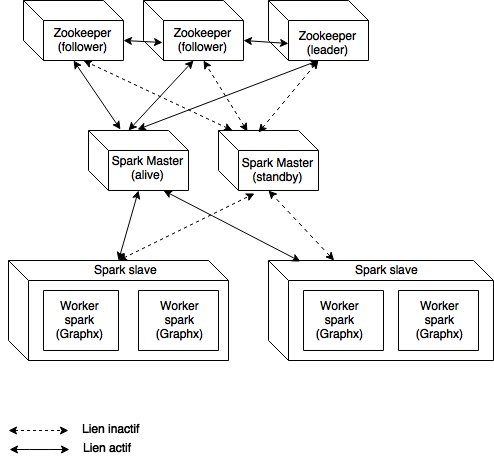
\includegraphics[scale=0.50]{pics/spark-infra.png}}
\centerline{\caption{Schéma globale de l'infrastructure mise en place pour SPARK}}
\ \\
\subsection{Haute disponibilité}
Pour permettre à notre cluster spark d'être résilient on va s'appuyer sur l'outils zookeeper. Il va nous permettre d'élire un leader entre les deux spark. Ainsi dans le cas où un leader meurt zookeeper se chargeras de basculer sur le second master spark en étant à jour le second master selon l'état du premier master. Cette opération de basculement entre les deux master peut prendre 1 à 2 minutes (le temps de détecter que le master spart est meurt et de mettre à jour l'état du second). Au niveau des workers spark gère lui même l'aspect resilience. Car comme dit plus haut si un worker tombe l'opération qui était en cours d'exécutions dessus seras lancé sur un nouveau worker par l'intermédiaire du master spark.


